% This is samplepaper.tex, a sample chapter demonstrating the
% LLNCS macro package for Springer Computer Science proceedings;
% Version 2.21 of 2022/01/12
%
\documentclass[runningheads]{llncs}
%
\usepackage[T1]{fontenc}
% T1 fonts will be used to generate the final print and online PDFs,
% so please use T1 fonts in your manuscript whenever possible.
% Other font encondings may result in incorrect characters.


% tightlist command for lists without linebreak
\providecommand{\tightlist}{%
  \setlength{\itemsep}{0pt}\setlength{\parskip}{0pt}}


% Pandoc citation processing
\newlength{\cslhangindent}
\setlength{\cslhangindent}{1.5em}
\newlength{\csllabelwidth}
\setlength{\csllabelwidth}{3em}
\newlength{\cslentryspacingunit} % times entry-spacing
\setlength{\cslentryspacingunit}{\parskip}
% for Pandoc 2.8 to 2.10.1
\newenvironment{cslreferences}%
  {}%
  {\par}
% For Pandoc 2.11+
\newenvironment{CSLReferences}[2] % #1 hanging-ident, #2 entry spacing
 {% don't indent paragraphs
  \setlength{\parindent}{0pt}
  % turn on hanging indent if param 1 is 1
  \ifodd #1
  \let\oldpar\par
  \def\par{\hangindent=\cslhangindent\oldpar}
  \fi
  % set entry spacing
  \setlength{\parskip}{#2\cslentryspacingunit}
 }%
 {}
\usepackage{calc}
\newcommand{\CSLBlock}[1]{#1\hfill\break}
\newcommand{\CSLLeftMargin}[1]{\parbox[t]{\csllabelwidth}{#1}}
\newcommand{\CSLRightInline}[1]{\parbox[t]{\linewidth - \csllabelwidth}{#1}\break}
\newcommand{\CSLIndent}[1]{\hspace{\cslhangindent}#1}

\usepackage[hidelinks]{hyperref}


\usepackage{graphicx}
% Used for displaying a sample figure. If possible, figure files should
% be included in EPS format.
%
% If you use the hyperref package, please uncomment the following two lines
% to display URLs in blue roman font according to Springer's eBook style:
\usepackage{hyperref}
\usepackage{color}
\renewcommand\UrlFont{\color{blue}\rmfamily}


\begin{document}


\title{Estimating the socio-environmental impacts of car substitution by
bicycle and public transit using open tools}
%
\titlerunning{Estimating the SE impacts of car substitution by bicycle
and public transit}
% If the paper title is too long for the running head, you can set
% an abbreviated paper title here
%
\author{Rosa Félix\inst{1}\orcidID{0000-0002-5642-6006} \and Filipe
Moura\inst{1}\orcidID{0000-0001-7749-8490} \and Robin
Lovelace\inst{2}\orcidID{0000-0001-5679-6536}}


\authorrunning{R. Félix et al.}
% First names are abbreviated in the running head.
% If there are more than two authors, 'et al.' is used.
%

\institute{CERIS - Instituto Superior Técnico, University of Lisbon. Av
Rovisco Pais 1049-001 Lisboa, Portugal\\
\email{\href{mailto:rosamfelix@tecnico.ulisboa.pt}{\nolinkurl{rosamfelix@tecnico.ulisboa.pt}}}\\ \and Institute
for Transport Studies, University of Leeds. 34-40 University Rd, Leeds
LS2 9JT, UK}

\maketitle              % typeset the header of the contribution
%
\begin{abstract}
In metropolitan areas, car trips can be replaced by a combination of
public transit and cycling for the first-and-last mile. This paper
focuses on estimating the potential for cycling + PT as a substitute for
car trips in the Lisbon metropolitan area and assessing its
socio-environmental impacts using open data and open source tools. A
decision support tool that facilitates the design and development of a
metropolitan cycling network was developed (\emph{biclaR}). A scenario
of intermodality introduced, and its socio-environmental impacts were
assessed using the \emph{HEAT for Cycling} and the \emph{HEAT as a
Service} tools. Additionally, the impacts of shifting car trips to PT
were estimated and monetized. The results indicate that 20\% of the
current trips can be made with the bicycle + PT combination. Shifting to
cycling for the first-and-last mile can reduce annual
CO\textsubscript{2}eq emissions from 6,000 tons/day, and the 10-year
socio-environmental benefits account from €230 million. For the PT leg,
the transfer from car results in the avoidance of at lest 8,500 tons of
CO\textsubscript{2}eq emissions per year. The information on
socio-economic benefits can support policymakers in prioritizing
interventions to reduce the reliance on individual motorized
transportation and effectively communicate their decisions.

\keywords{Active transport \and Intermodality \and First and last
mile \and Health economic assessment \and Environmental
impacts \and Open data and methods}

\end{abstract}

\hypertarget{introduction}{%
\section{Introduction}\label{introduction}}

\textbf{full paper}: 4-6 pages in length (typically up to 3,000 words).

In metropolitan areas, car trips can be replaced by a combination of
public transit (PT) and cycling for the first-and-last mile. This
approach requires interventions and programs to make bicycling more
appealing, and the resulting public investments can have significant
social and environmental benefits. This paper focuses on estimating the
potential for cycling + PT as a substitute for car trips in the Lisbon
metropolitan area (LMA) and assessing its socio-environmental impacts
using open data and open source tools.

According to the latest mobility survey conducted in 2018, the LMA
registered a total of 5.3 million daily trips, with only 0.5\% by
bicycle. Car modal share is 58.4\%, while PT accounts for 15.5\%. To
achieve the cycling targets set by the Portuguese national cycling
strategy for 2025 and 2030 (4\% and 10\%, respectively), the Department
of Transport introduced biclaR, a decision support tool that facilitates
the design and development of a metropolitan cycling network.

This research aims to present and discuss the methods used to
estimate\ldots{}

Propensity to Cycle Tool

adding up an intermodality scenario to estimate cycling potential to
public transit interfaces, and thus to support planning and prioritize
investments in the cycling network.

\hypertarget{methods}{%
\section{Methods}\label{methods}}

\hypertarget{case-study}{%
\subsection{Case Study}\label{case-study}}

As características das viagens do IMob, constituem o cenário base deste
projeto. Este inquérito à mobilidade foi realizado em 2017. Apesar de
ter sido realizado em período pré-pandemia, este conjunto de dados é a
melhor e mais recente informação que temos em termos de mobilidade
urbana nas áreas metropolitanas.

Segundo o IMob (2017), das cerca de 5.3 milhões de viagens diárias na
área metropolitana de Lisboa, apenas 25 479 das viagens são realizadas
em bicicleta (0,5\%), enquanto 3.1 milhões são feitas em automóvel
(58.4\%), 1.3 milhões a pé (23.9\%), 825 mil em transportes públicos
(15.5\%) e 96 mil em outros modos (1.8\%).

O número de viagens intramunicipais - ou que são realizadas com origem e
destino no mesmo município (3.5 milhões viagens) - é superior ao número
de viagens intermunicipais - com origem e destino em municípios
diferentes (1.8 milhões viagens). O automóvel e os transportes públicos
são os modos maioritariamente utilizados em viagens intermunicipais. O
automóvel é o modo mais utilizado em qualquer tipologia de viagem.

Este é o cenário base, ou de referência, utilizado apenas para
comparação com os cenários seguintes - de onde advém o potencial
ciclável.

\hypertarget{modeling-origin-destination-trips}{%
\subsection{Modeling Origin-Destination
trips}\label{modeling-origin-destination-trips}}

imob data

Aplicou-se um método de desagregação das origens e destinos das viagens
entre o centróide de uma freguesia para o centróide de outra freguesia,
para que uma freguesia não esteja representada apenas por um único local
de origem e destino das suas viagens (centróides).

Ao agregar as viagens todas em centróides, tornamos o exercício menos
realista pois elimina um conjunto importante de viagens de curta
distância, o que é uma característica de viagens em modos ativos
(\textbf{ref2?}). Para tal, recorreu-se ao método OD Jittering, que
utiliza uma desagregação de um único ponto (por exemplo o centróide de
uma área) em vários pontos aleatórios da rede viária existente, com base
no OpenStreetMap, e divide o volume de viagens dessa freguesia pelos
pares origem-destino gerados aleatoriamente.

Para este projeto, utilizou-se um nível de desagregação máxima de 100
viagens por par O-D. Isto significa que, por exemplo, para um par O-D de
2.000 viagens entre duas freguesias ligadas entre os seus centróides, o
método jittering dispersa aleatoriamente as 2.000 viagens em 20 pares de
100 viagens entre 20 origens e 20 destinos nas duas freguesias.

A figura 3 ilustra a diferença entre a representação de viagens
utilizando o método tradicional de ligação entre um único local entre
cada freguesia, e a representação com a aleatorização e desagregação de
viagens entre freguesias, para a área metropolitana de Lisboa. Figura 3
- Representação de pares OD na área metropolitana de Lisboa entre
freguesias, sem jittering (à esquerda), e com jittering (à direita).

O resultado da utilização deste método, em vez do tradicional uso de
centróides de grandes áreas, é que torna mais realistas a representação
de viagens realizadas, não correspondendo, no entanto, aos pares O-D
reais das viagens realizadas (por motivos de proteção de dados definidos
pelo INE). Para uma melhor compreensão do método utilizado, consultar
Jittering: A Computationally Efficient Method for Generating Realistic
Route Networks from Origin-Destination Data (Lovelace, Félix, and
Carlino 2022)

\hypertarget{modeling-routes}{%
\subsection{Modeling routes}\label{modeling-routes}}

A identificação dos percursos entre as origens e destinos (para as
linhas de desejo) são um aspeto fundamental da modelação da rede
ciclável nesta metodologia, uma vez que o IMob não identifica os
percursos realizados por cada viagem, sendo necessário estimá-los. A
respetiva modelação depende do cenário escolhido e tem em conta toda a
restante informação disponível (como os declives, ou localização de
interfaces de transporte público), para além da informação viária base.

A partir das linhas de desejo do cenário base, traçam-se os percursos
modelados para o modo ciclável com base na rede viária (equivalente à
afetação das viagens à rede, 4.º e último passo do modelo clássico dos 4
passos em sistemas de transportes). A modelação dos percursos cicláveis
depende das variáveis consideradas, assim como das restrições
pré-definidas. Estas restrições podem privilegiar aspetos como
velocidade e volumes baixos, rotas mais diretas, percursos menos
declivosos, entre outros, adequados à utilização da bicicleta, sendo que
o algoritmo segue uma avaliação que resulta da ponderação das variáveis
consideradas. Mesmo o percurso menos declivoso, mas com maior volume de
tráfego, poderá ser o indicado se a função assim o definir.

O algoritmo de escolha de percurso escolhido foi o do r5r que é um
algoritmo que permite muita flexibilidade nas configurações de tipo de
percursos estimados, nomeadamente por permitir estimar com probabilidade
e incerteza os percursos que usam transportes públicos (considerando os
seus horários). O r5r permite a identificação de percursos mais diretos
ou mais seguros, recorrendo para isso ao nível de stress de tráfego
(Level of Traffic Stress, ou LTS), que varia de 1 a 4, sendo o 1 mais
tranquilo - correspondendo, por exemplo, a pistas cicláveis fora de
estrada, e o 4 menos tranquilo - correspondendo, por exemplo, a
percursos que partilham o tráfego motorizado. Os percursos foram
estimados para o cenário base, para ambos os tipos de rede, direto e
seguro, usando para isso o LTS 4 e LTS 3 respetivamente.

O nível de tranquilidade\footnote{see
  \url{https://www.cyclestreets.net/help/journey/howitworks/\#quietness}}
é outro indicador estimado pelo CycleStreets para cada troço, com base
no número de vias, velocidade máxima permitida, arborização, hierarquia
e tráfego (quando a informação correspondente existe nas etiquetas do
OpenStreetMap). É apresentado numa escala de 0 a 100, em que o zero
corresponde ao nível menos seguro para se circular de bicicleta, e o 100
ao nível mais seguro e tranquilo - normalmente correspondendo a troços
que incluem já infraestrutura ciclável segregada do tráfego motorizado.

Foi utilizado um modelo digital do terreno de 25m de resolução espacial
e erro médio de altimetria vertical de 2.12m8 em Portugal, da Agência
Espacial Europeia, na sua missão COPERNICUS, para incluir impedâncias 9
de declives no modelo. O modelo r5r utiliza a rede viária do
OpenStreetMap (extraída a 22 de outubro 2022), e os dados de GTFS
criados e validados para o efeito. Foi estimado o número de viagens em
bicicleta potencial para as duas metas ENMAC (5\% e 10\%) a partir dos
valores de viagens em bicicleta e em automóvel (como condutor e como
passageiro) do cenário base de 2017.

Os percursos ou rotas foram depois sobrepostos e agregados por
segmentos, juntando a informação de várias rotas que se sobrepõem em
certos segmentos (overline). Por exemplo, foram somados os volumes de
viagens em bicicleta estimados e a transferência do automóvel, e foi
feita a média da velocidade automóvel e do nível de tranquilidade,
ponderadas pela distância dos segmentos.

\hypertarget{modeling-intermodality}{%
\subsection{Modeling intermodality}\label{modeling-intermodality}}

The intermodality scenario considers trips that can combine PT and
cycling for the first-and-last legs. Conservatively, we considered the
sum of first-and-last legs up to 5 km. Furthermore, we restricted PT use
to unimodal trips without transfers (although they can be included in
future modeling). Félix, Lovelace, and Moura (2022)

Finally, we only included PT modes that can practically accommodate
bicycles, such as trains, ferries, trams, and intermunicipal bus lines
with bike racks (~\ref{fig:map1}).

Foram recolhidos os dados de transportes públicos da AML, em formato
GTFS, tendo sido necessário o trabalho de limpeza, união, e validação
prévio. Esta informação é indispensável para saber que terminais de
transporte público (TP) se ligam a que origens ou destinos, e em que
horários, para não se considerar de forma generalista que uma interface
se liga a todo o sistema e que pode servir todas as viagens (origens e
destinos), o que não seria realista.

\begin{figure}
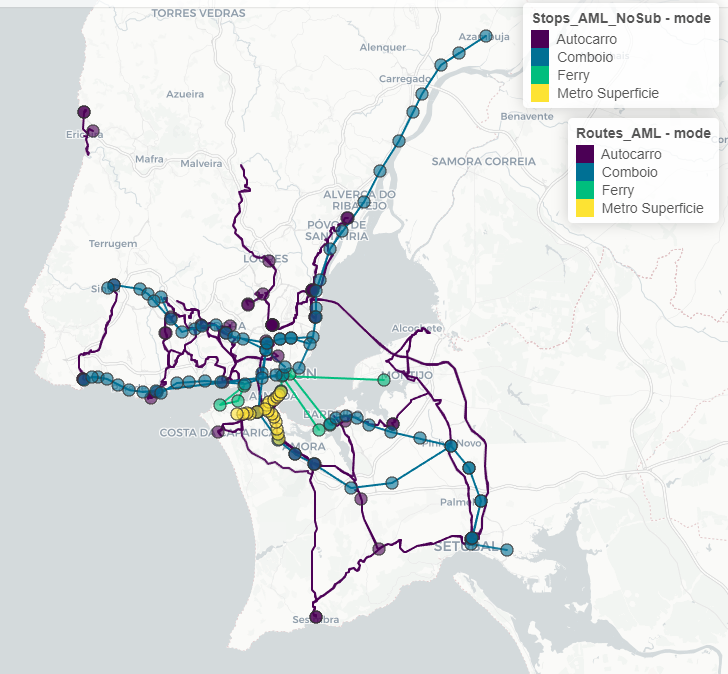
\includegraphics[width=0.6\linewidth,]{img/map1} \caption{Interfaces and lines considered, by transport mode, in the Lisbon metropolitan area}\label{fig:map1}
\end{figure}

To obtain reliable results, we used the OpenStreetMap road network and
GTFS data. The r5r R package estimated the trip duration and distance
for both the original modes and the bicycle + PT combination, while the
od jittering R package estimated the OD locations based on a
centroid-based OD matrix.

Para a modelação dos percursos definiu-se como janela temporal viagens
até 120 minutos (2h). Para além disso considerou-se como duração máxima
25 minutos em bicicleta.

Map result (~\ref{fig:map2}).

\begin{figure}
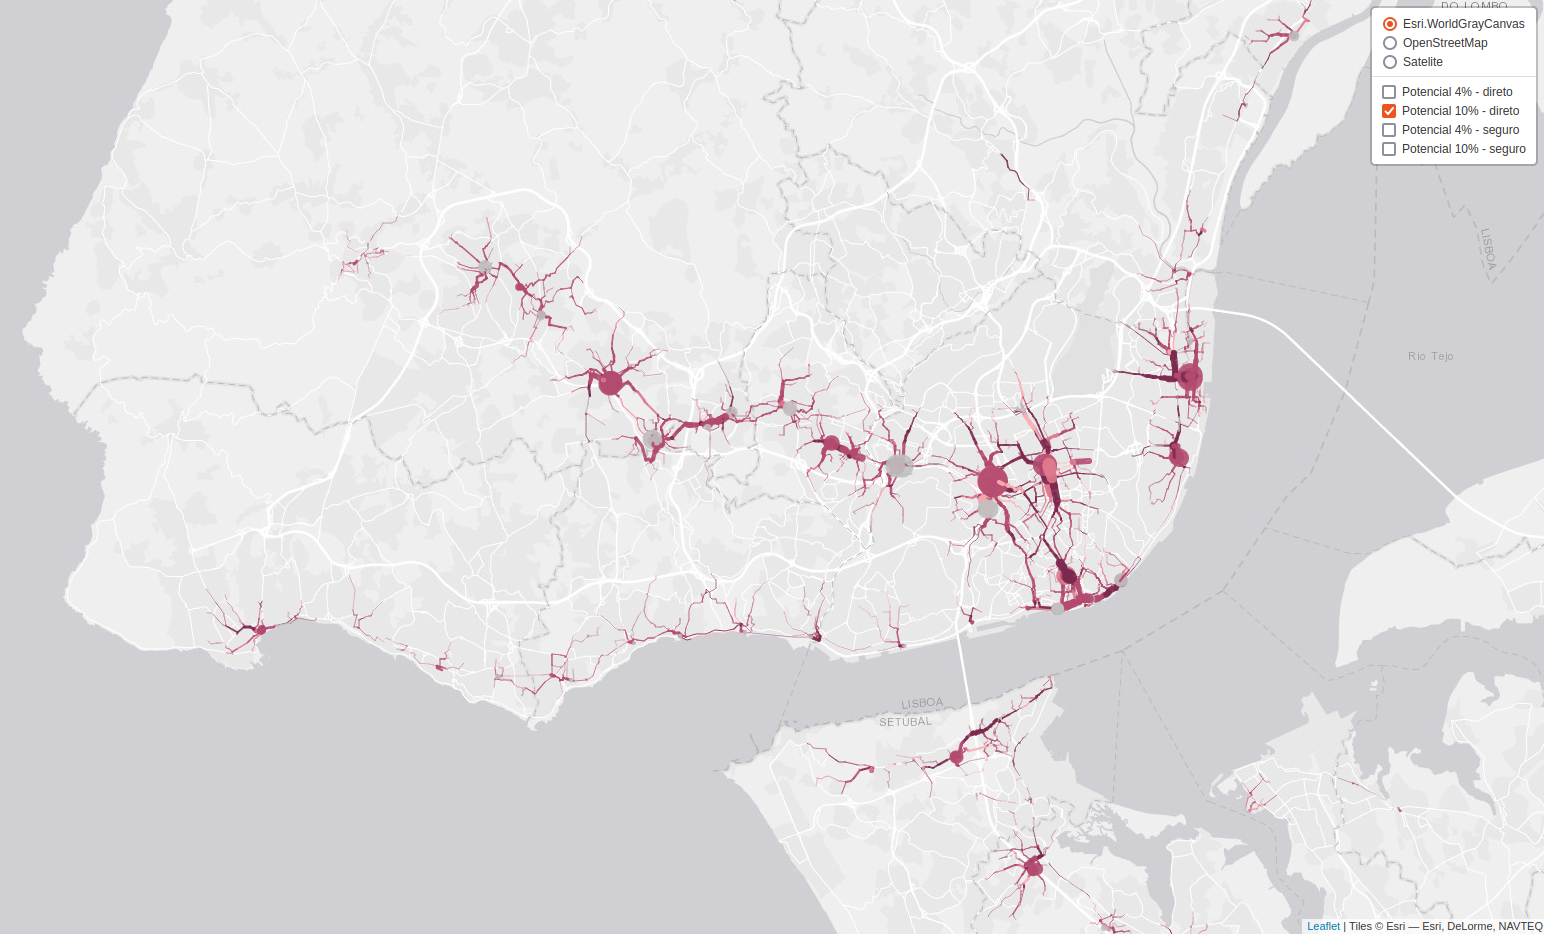
\includegraphics[width=0.8\linewidth,]{img/map2} \caption{Bike routes with highest potential to serve as first and last mile when replacing cycling and PT from car trips (screenshot of the interactive online tool).}\label{fig:map2}
\end{figure}

\hypertarget{assessing-socio-environmental-benefits}{%
\subsection{Assessing socio-environmental
benefits}\label{assessing-socio-environmental-benefits}}

Socio-environmental impacts were assessed using the HEAT for Cycling and
the HEAT as a Service\footnote{see
  \url{https://github.com/HEAT-WHO/HEAT_heatr_api}} tools, from the WHO.
Additionally, we estimate the impacts of shifting car trips to PT for
the second leg of the journey with EMEP/EEA's COPERT methodology and
monetize them with the EU Guide to cost-benefit analysis.

Como referido na introdução, a ferramenta biclaR pretende estimar os
impactes sociais e ambientais associados ao potencial ciclável dos
vários cenários analisados. O horizonte temporal considerado para esta
análise foi o curto prazo (i.e., 1 ano) e o longo prazo (i.e., 10 anos).
Os impactes foram avaliados para cada cenário e para diferentes escalas
territoriais:

\begin{itemize}
\tightlist
\item
  Desagregado à escala municipal para cada segmento de rede:

  \begin{itemize}
  \tightlist
  \item
    Ambientais (emissões de CO\textsubscript{2}eq evitadas);
  \item
    Balanço monetarizado dos impactes socioeconómicos totais
    (considerando o balanço dos impactes ambientais e sociais);
  \end{itemize}
\item
  Agregado à escala metropolitana:

  \begin{itemize}
  \tightlist
  \item
    Ambientais (emissões de CO\textsubscript{2}eq evitadas);
  \item
    Balanço monetarizado dos impactes socioeconómicos totais
    (considerando o balanço dos impactes ambientais e sociais);
  \item
    Ambientais (emissões de CO\textsubscript{2}eq, CO, PM10, NOx, e
    VOC11, evitadas por substituição dos modos motorizados, considerando
    as emissões geradas na transferência para transportes públicos).
  \end{itemize}
\end{itemize}

Para todos os cenários, recorreu-se à ferramenta HEAT for cycling, da
Organização Mundial de Saúde, para estimativa dos impactes sociais e
ambientais da transferência de viagens em automóvel para viagens em
bicicleta, nas componentes de: a) Social - Saúde, Atividade Física,
Exposição a poluição atmosférica, Exposição ao risco de sinistralidade
rodoviária; b) Ambiental - Emissão de gases CO\textsubscript{2}eq.

A estimativa dos impactes ambientais resulta em toneladas de
CO\textsubscript{2}eq, e a estimativa dos impactes sociais resulta em
mortalidade prematura evitada. Ambas as unidades são por fim monetizadas
em €, segundo os valores da literatura utilizada em estudos semelhantes.
Para além dos impactes sociais e ambientais resultantes da transferência
do automóvel para a bicicleta (na primeira e na última parte da viagem,
de e para a interface de TP), estimou-se também o impacte ambiental
adicional, resultante da transferência do automóvel para os vários
transportes públicos (na segunda etapa da viagem, entre as interfaces).
Como tal, foi necessário caracterizar o universo dos modos motorizados a
serem considerados para os cálculos dos respetivos fatores de emissões
de gases poluentes e atmosféricos.

Os fatores de consumo e de emissão dos automóveis e transportes públicos
deve ser tido em conta relativamente ao número de passageiros
transportados (por passageiro.km) e não ao veículo (que seria
veículo.km). No caso do automóvel, para contabilizar a emissão de gases
evitados pela transferência de viagens em automóvel para os transportes
públicos, teve-se em conta o valor de referência de 1.61
passageiros/automóvel reportados pelo Inquérito à Mobilidade (INE 2017).

As emissões evitadas por cada viagem em transportes públicos que
substitui o automóvel correspondem às emissões equivalentes de um
automóvel com características correspondentes à média da frota em
circulação em Lisboa, para 2 tipos de combustível: gasolina e gasóleo.
Utilizou-se a metodologia e valores de referência do software COPERT
(Ntziachristos and Samaras 2020), v5.0, da Agência Europeia do Ambiente,
para um nível de detalhe 3 (Tier 3) na estimativa de consumo de emissões
para o automóvel, nestes dois tipos de combustível. Optou-se por usar um
veículo de dimensão familiar, norma EURO, e tipo de combustível gasolina
ou diesel. Considerou-se que as viagens foram todas realizadas em
condições urbanas (com as respetivas implicações no regime médio de
condução) e a uma velocidade média de 15km/h, nos períodos de hora de
ponta. Uma vez que a distância média percorrida por viagem influencia o
nível de sobreconsumo e emissões decorrentes da operação do motor a frio
-- ou seja, distâncias maiores diluem a importância deste sobreconsumo
face ao fator de consumo com o motor a operar a quente, foram estimados
os consumos para diferentes gamas de viagem, em intervalos de 500
metros. As emissões são estimadas para os seguintes poluentes
atmosféricos: CO (monóxido de carbono), NO X (Óxidos de Azoto), COV
(Compostos Orgânicos Voláteis), PM (material particulado). Também é
estimada as emissões dos principais gases com efeito de estufa: CO2
(dióxido de carbono); CH4 (metano) e N2O (Óxido nitroso), assim como o
CO\textsubscript{2}eq equivalente.

Relativamente aos transportes públicos, recorreu-se aos fatores de
emissão reportados nos relatórios de sustentabilidade dos respetivos
operadores (Carris 2020; Metropolitano de Lisboa 2020; CP 2020, Grupo
Transtejo 2014).

a conversão das emissões evitadas em perda de bem-estar evitado, através
da respetiva valorização monetária. a partir dos valores de referência
para os vários gases contabilizados, atualizados para 2022 15, com base
nas fontes: Bickel et al.~(2006), Nash and others (2003), Sartori et
al.~(2014).

\hypertarget{results-and-discussion}{%
\section{Results and Discussion}\label{results-and-discussion}}

A Tabela 4 apresenta o número de viagens diárias do cenário base e
potenciais, passíveis de serem realizadas até 5 km em bicicleta em
complemento com TP, por tipo de percurso. Para as redes segura e direta,
as viagens do cenário base até 5 km em bicicleta + TP correspondem a
20\% do total de viagens reportadas no inquérito.

Este cenário valoriza a utilização da bicicleta como complemento ao
transporte público, com potencial de aumentar as viagens em TP
realizadas na área metropolitana de Lisboa em até 12\% (acrescentando às
825 mil do IMob 2017). Estes resultados sugerem que o potencial de
transferência de viagens em automóvel para bicicleta + TP poderá ser
quase ou tão importante quanto a transferência para viagens utilizando
apenas a bicicleta.

Para este cenário foram estimados os impactes ambientais de
transferência do automóvel para os transportes públicos, para além dos
impactes ambientais e sociais da transferência para a bicicleta

Foram então calculadas as emissões dos poluentes para cada viagem
substituída, tendo em conta o modo de transporte, distâncias e
velocidade. A tabela 11 apresenta a estimativa anual de gases emitidos e
evitados por transferência do automóvel para os outros modos de
transporte público, como exemplo para o cenário com a meta de 4\%,
usando a rede ciclável ``direta''.

{[}Tabela 11{]}

Para esse cenário com essas características, é estimada uma poupança de
8 702 toneladas de CO\textsubscript{2}eq por via da transferência de
viagens motorizadas com combustíveis fósseis e eletricidade, numa
perspetiva de ciclo de vida da produção de eletricidade.

A valorização monetária das emissões (em toneladas) é apresentada na
tabela seguinte, para o cenário 3 (apenas a segunda parte da viagem, em
transportes públicos), com as metas de 4\% e 10\%, e usando as redes
cicláveis ``direta'' e ``segura'', para 365 dias (1 ano).

{[}Tabela 13{]}

\begin{figure}
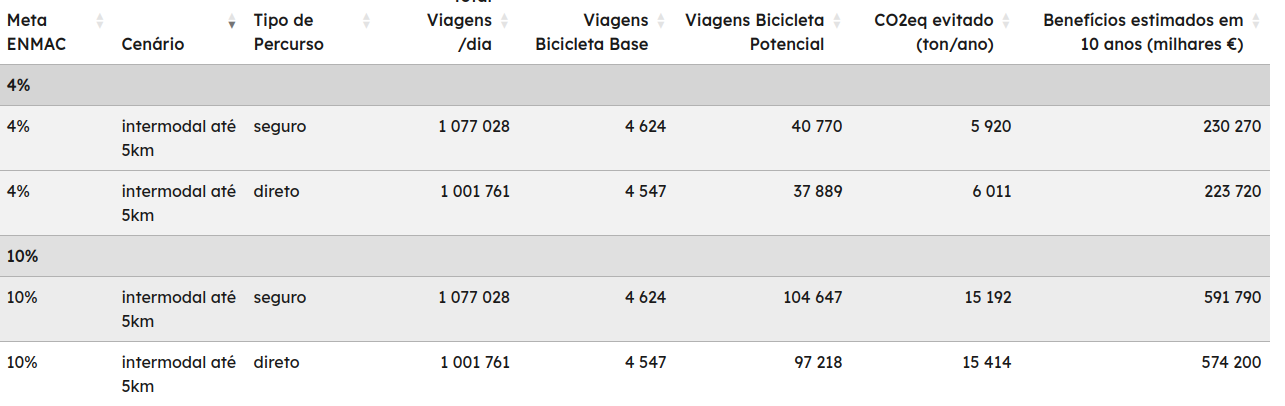
\includegraphics[width=1\linewidth,]{img/table1} \caption{Summary of the cycling potencial of intermodality scenario.}\label{fig:summary1}
\end{figure}

\begin{figure}
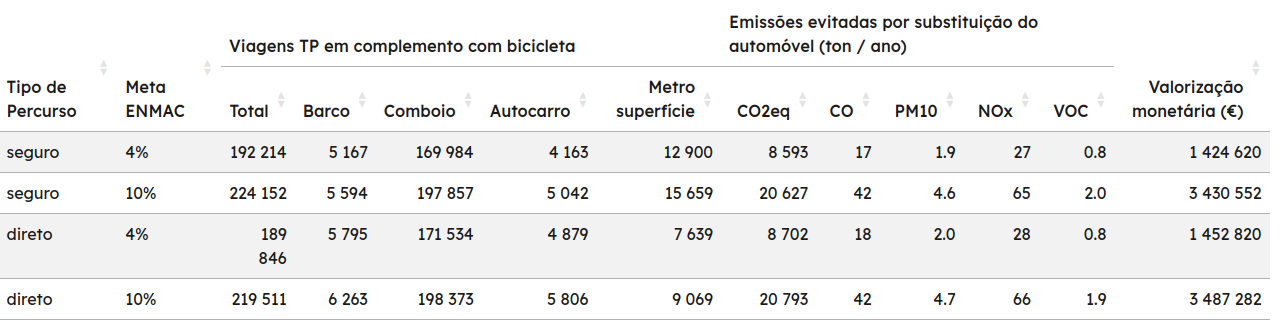
\includegraphics[width=1\linewidth,]{img/table2} \caption{Potencial de transferência estimado para cada modo de transporte público, bem como as estimativas de consumo de CO~2~eq evitado anualmente por transferência do automóvel.}\label{fig:summary2}
\end{figure}

Em suma, o impacte socioeconómico das emissões de gases poluentes e de
gases de efeito estufa pode ser valorizado numa poupança potencial de
entre 1.4 a 3.5 milhões €, a acrescentar aos impactes estimados na
secção anterior.

The results indicate that 20\% of the current trips can be made with the
bicycle + PT combination, with an additional 12\% of PT trips being
potentially replaced. Shifting to cycling for the first-and-last mile
can reduce annual CO\textsubscript{2}eq emissions by 6,000 to 15,000
tons/day, and the 10-year socio-environmental benefits account for €230
to €590 million, depending on the cycling targets. For the PT leg, the
transfer from car results in the avoidance of 8,500 to 20,800 tons of
CO\textsubscript{2}eq emissions per year, or €1.4 to €3.5 million over
10 years, with trains offering the greatest potential for substitution
(88\%).

\hypertarget{conclusion}{%
\section{Conclusion}\label{conclusion}}

By making the research process publicly accessible in a code repository,
this study enables the replication of similar estimates for
socio-environmental impacts resulting from a modal shift from cars to
bicycles + PT in other metropolitan areas. The provided information on
socio-economic benefits can support policymakers in prioritizing
interventions to reduce the reliance on individual motorized
transportation and effectively communicate their decisions.

\hypertarget{acknowledgements}{%
\subsubsection*{Acknowledgements}\label{acknowledgements}}
\addcontentsline{toc}{subsubsection}{Acknowledgements}

Please place your acknowledgments at the end of the paper, preceded by
an unnumbered run-in heading (i.e.~3rd-level heading).

Thomas Götshi - HAAS.

\hypertarget{references}{%
\section*{References}\label{references}}
\addcontentsline{toc}{section}{References}

\hypertarget{refs}{}
\begin{CSLReferences}{1}{0}
\leavevmode\vadjust pre{\hypertarget{ref-felix2023}{}}%
Félix, Rosa, Robin Lovelace, and Filipe Moura. 2022. {``{biclaR -
Ferramenta de apoio ao planeamento da rede ciclável na área
metropolitana de Lisboa}.''} {CERIS - Instituto Superior Técnico and
Transportes Metropolitanos de Lisboa}.
\url{https://biclar.tmlmobilidade.pt}.

\leavevmode\vadjust pre{\hypertarget{ref-bib2}{}}%
Slifka, M. K., and J. L. Whitton. 2000. {``Clinical Implications of
Dysregulated Cytokine Production.''} \emph{J. {M}ol. {M}ed.} 78: 74--80.
\url{https://doi.org/10.1007/s001090000086}.

\end{CSLReferences}

%
% ---- Bibliography ----



\end{document}
